\documentclass{beamer}

% import packages
\usepackage[T1]{fontenc}
\usepackage{lmodern}
\usepackage[a0paper]{beamerposter}
\usepackage{graphicx}
\usepackage{booktabs}
\usepackage{tikz}
\usepackage{pgfplots}
\usepackage{anyfontsize}
\usepackage{siunitx}
\usepackage{multicol}
\usepackage{subcaption}

% configure pgfplots
\pgfplotsset{compat=1.14}

% specify theme and color theme
\usetheme{gemini}
\usecolortheme{earth}

% define poster lengths for columns
% If you have N columns, choose \sepwidth and \colwidth such that
% (N+1)*\sepwidth + N*\colwidth = \paperwidth
\newlength{\sepwidth}
\newlength{\colwidth}
\setlength{\sepwidth}{0.025\paperwidth}
\setlength{\colwidth}{0.3\paperwidth}
% define the separator column command
\newcommand{\separatorcolumn}{\begin{column}{\sepwidth}\end{column}}

% configure the author block
\title{Microtubule force generation in axon growth cones}
\author{Calvin Sprouse}
\institute[CWU]{Department of Physics, Central Washington University}

% configure the footer
\footercontent{
    PHYS 322 Computational Biophysics \hfill
    2024 March 12 \hfill
    \href{mailto:calvin.sprouse@cwu.edu}{calvin.sprouse@cwu.edu}
}

% setup logo
\logoright{
\includegraphics[height=7cm]{figures/logos/cwu_logo.png}}


%-----------------------------------------------------------------------------%
% begin poster
\begin{document}

% begin the content framework
\begin{frame}[t]
\begin{columns}[t]
\separatorcolumn%


%-----------------------------------------------------------------------------%
% first column of content
\begin{column}{\colwidth}

%------------------------------------------------
% introduction/abstract block
\begin{block}{Introduction}

The neuron is a class of living cell adapted to function as a network node. Neurons have two types of protrusion from their cell body which begin as neurites. Most neurites become dendrites, which are smaller branches that support bidirectional transport of both signal and cargo. They also serve as targets for incoming network connections from other neurons. One neurite on each neuron becomes the axon. This longer branch is adapted to support outbound signaling from the cell body. While the dendrites remain relatively close to cell body the axon grows following chemical cues. The rate of axon growth varies by the function of the neuron and can extend from micrometers to meters.

Besides its length, the axon expresses unique internal traits from the dendrite. Most notably is the emergent ordering of microtubule (MT) filaments in the axon~\cite{nedelec_self-organization_1997}. MTs are dynamic assemblies of tubulin that serve as molecular highways. The plus-end of an MT is where most polymerization activity occurs. The polarity of an MT is its relative orientation in the context of the cell body. Molecular motors are sensitive to polarity as each motor has a directional preference. Dynein, for example, is a minus-directed motor and walks away from the plus-end. Kinesin, on the other hand, is a plus-directed motor. The polarity pattern describes the spatial distribution of MT polarity and indicates the function of the region.

\begin{figure}
    \centering
    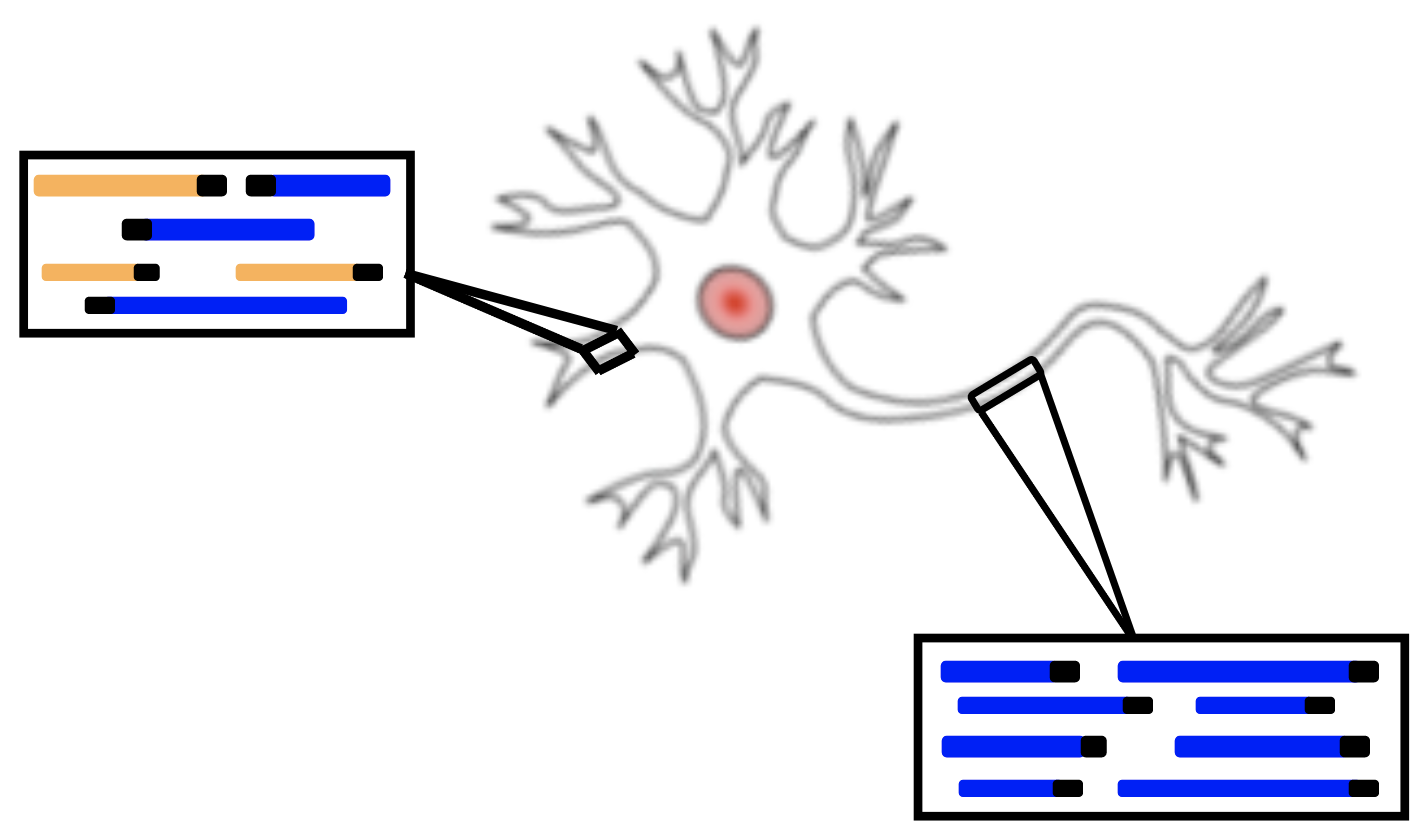
\includegraphics[width=0.5\textwidth]{figures/background/neuron_with_mts.png}
    \caption{\label{fig:neuron_background}
        A neuron with dendrites and an axon extending from the cell body. MTs are shown in two regions: left is a dendrite, and right is an axon. The plus-end of the MTs is indicated by a black rectangle. The orientation of the MTs with respect to the cell body is indicated by the color: blue MTs are plus-end-out, orange MTs are minus-end-out.}
\end{figure}

The axon shown in Figure~\ref{fig:neuron_background} expresses the typical plus-end-out polarity pattern whereas the dendrite exhibits a typical mixed polarity pattern.

\end{block}

\begin{block}{Background}

\begin{figure}
    \centering
    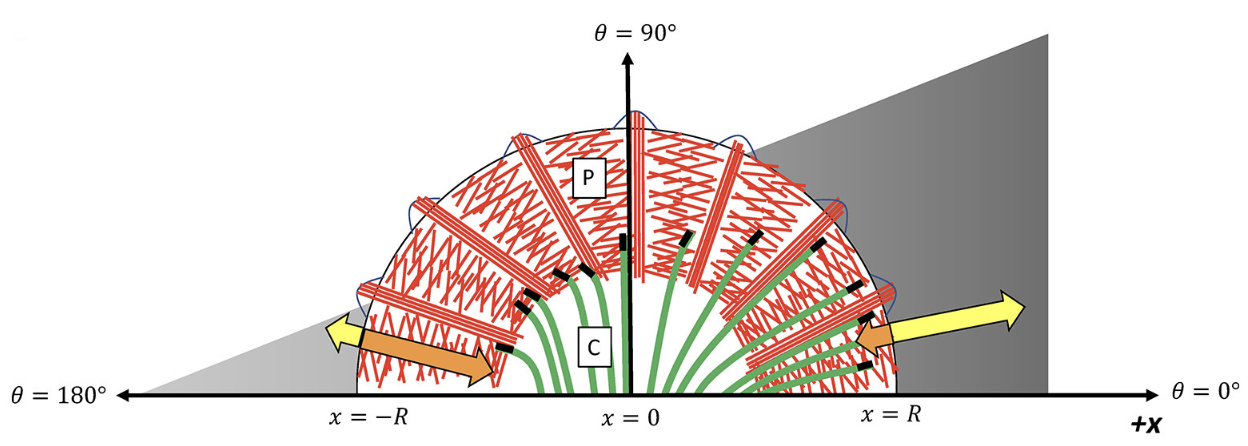
\includegraphics[width=0.65\textwidth]{figures/introduction/gc_crag_1a.png}
    \caption{\label{fig:gc_craig}
        Illustrative schematic of a growth cone from Ref.~\cite{craig_model_2018} Figure 1A. Shown in green with black tips are the MTs as in Figure~\ref{fig:neuron_background}. Shown in black is a chemical gradient indicating the direction the GC should steer. Yellow and orange arrows indicate the relative velocity of forward polymerization and depolymerization respectively of the actomyosin network. The presence of MTs increases adhesion of the actomyosin network and promotes forward polymerization.
    }
\end{figure}

Axon growth is lead by a region called the growth cone (GC) shown in Figure~\ref{fig:gc_craig}. The GC is distinguished from the rest of the axon by a decrease in MT density, sensing equipment for reading chemical guidance cues, and a force generating network of actin filaments and myosin motors.

\begin{figure}
    \centering
    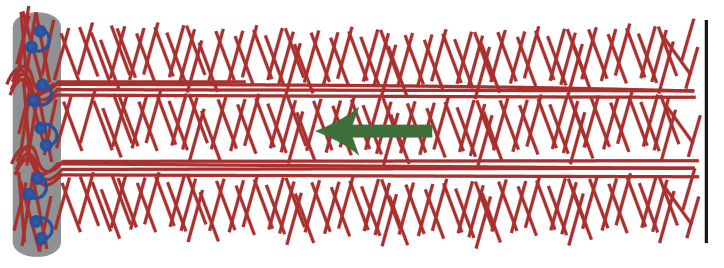
\includegraphics[width=0.4\textwidth]{figures/introduction/actin_treadmill.png}
    \caption{\label{fig:actin_craig}
        Actin treadmill schematic from Ref.~\cite{craig_membrane_2012} Figure 1B. This view is effectively a thin angular slice of Figure~\ref{fig:gc_craig}. The rightmost edge is the leading edge of the GC where polymerization activity occurs. The leftmost edge then houses the depolymerization machinery.
    }
\end{figure}

The actomyosin network is a treadmill of actin filaments and myosin motors thought to be the primary diver in elongation~\cite{craig_membrane_2012}. The treadmill behavior emerges from the combination of leading edge polymerization and trailing edge depolymerization of the actin shown in Figure~\ref{fig:actin_craig}. Also impacting the actomyosin network are tension forces from the stretching of the GC membrane~\cite{craig_membrane_2012}. Myosin acts simultaneously as a crosslinker for the network and the transporter of trailing edge depolymerize actin filament to the leading edge for polymerization. By modulating actin adhesion to the substrate the GC can execute carefully controlled growth and steering. The role of MTs is currently understood as signal pathways between the chemical sensing equipment and the actomyosin network~\cite{craig_membrane_2012, kalil_touch_2005,sanchez-huertas_permission_2021}.

\begin{figure}
    \centering
    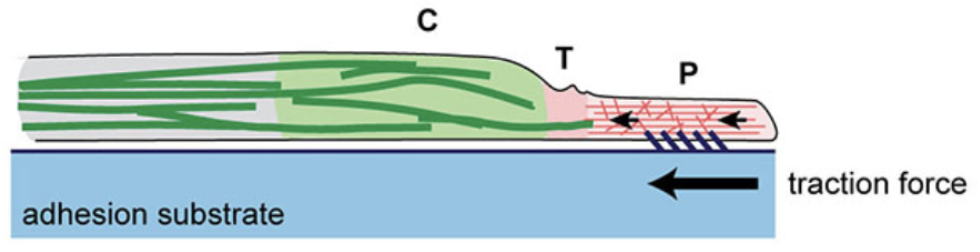
\includegraphics[width=0.5\textwidth]{figures/introduction/traction_generation.png}
    \caption{\label{fig:traction}
        A side-view schematic of the GC from Ref.~\cite{athamneh_quantifying_2015} Figure 1. Shown in green are the MTs as in Figure~\ref{fig:neuron_background}. This is representative of our proposed one-dimensional model. Black arrows indicate the direction of actin flow and generated forces from the GC frame.
    }
\end{figure}

We investigate the role of the MTs in the GC regions as conveyors of force from the axon. In the axon, Dynein motors act between MTs inducing \(\qty{}{\pico\newton}\) scale forces primarily in the direction of the MTs plus-end~\cite{nedelec_self-organization_1997, raffa_force_2023}. The forces acting on the GC are observed to be small, on the order of \(\qty{}{\pico\newton}\)~\cite{de_vincentiis_extremely_2020, raffa_force_2023}. Furthermore, it seems the MTs protruding into the GC act to stabilize against contractile forces generated in the actomyosin network and the GC membrane~\cite{raffa_force_2023}. We extend the work done in Ref.~\cite{craig_membrane_2012} to include distill-end MT force generation by a Dynein sorting mechanism and investigate the consequence of interaction in the GC.

\end{block}

\end{column}
\separatorcolumn%


%-----------------------------------------------------------------------------%
% second column of content
\begin{column}{\colwidth}

%------------------------------------------------
% content block
\begin{block}{Model}

We begin with Ref.~\cite{craig_membrane_2012} which describes a one-dimensional computational adhesion clutch model in the context of the actomyosin network. This is a population based steady-state model which aims to explore the relationship of actin retrograde flow, actin density, and traction forces.

% "default" figure from simulation showing exactly this relationship
% \begin{figure}
%     \centering
%     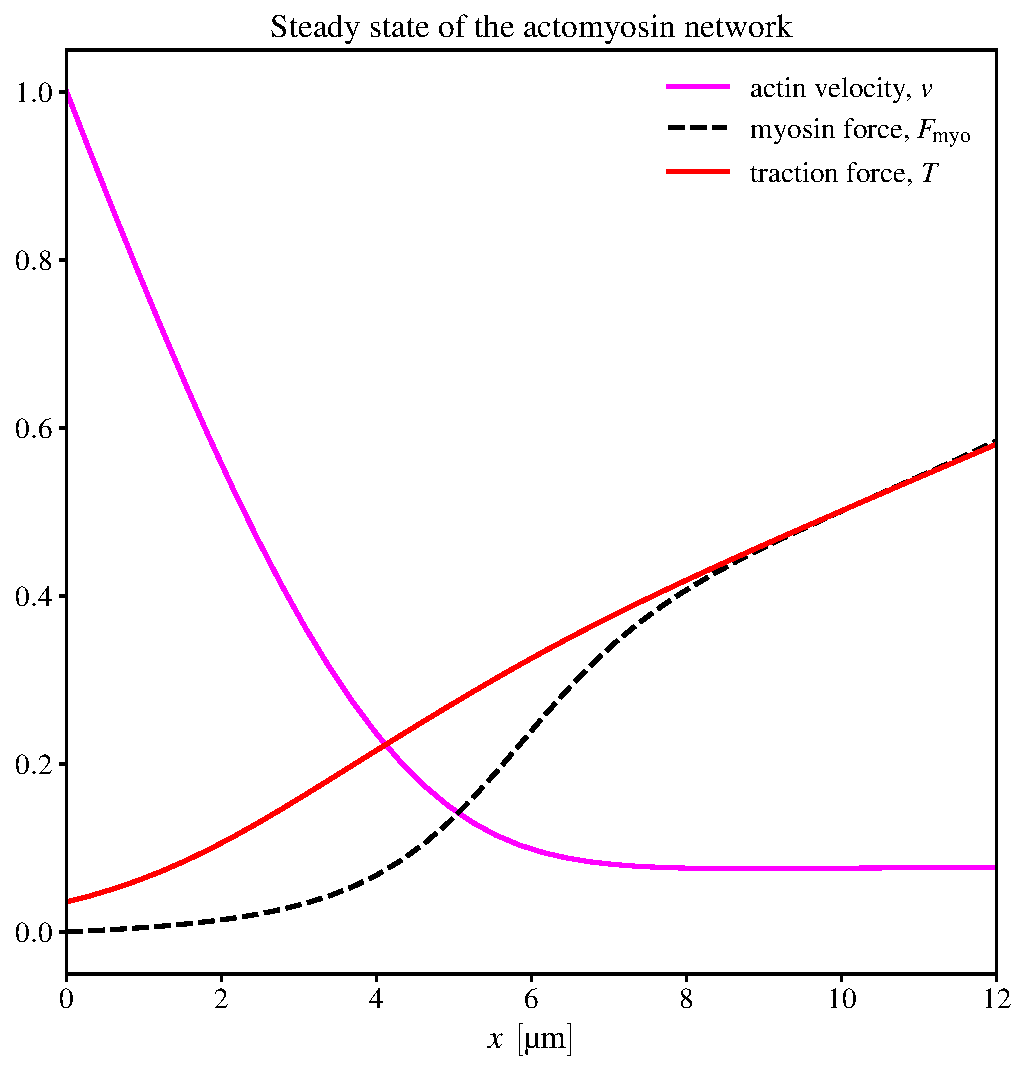
\includegraphics[width=0.35\textwidth]{../.figures/steady_state_og.pdf}
%     \caption{\label{fig:sim_steady}
%         Representative output of the steady state of the actomyosin network from Ref.~\cite{craig_membrane_2012}. The pink line represents the retrograde actin flow speed from the leading edge, \(x=\qty{0}{\micro\meter}\), to the trailing edge, \(x=\qty{12}{\micro\meter}\). The black dashed line represents the contractile forces from myosin. The red line represents the traction forces arising from actin adhesion to the substrate. Under these conditions the GC is moving in the \(-x\) direction.
%     }
% \end{figure}

\begin{figure}
    \begin{subfigure}{0.3\textwidth}
    \centering
    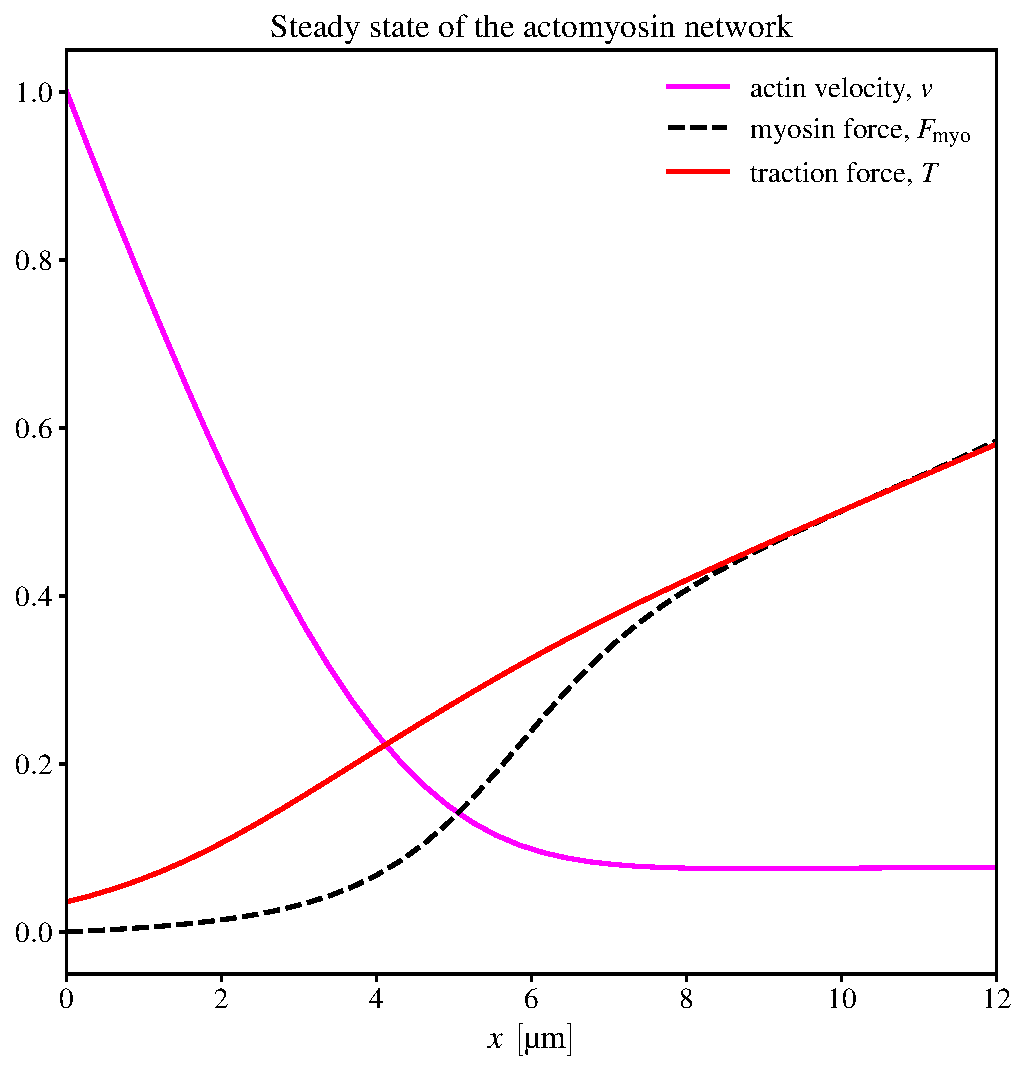
\includegraphics[width=\linewidth]{../.figures/steady_state_og.pdf}
    \caption{\label{fig:steady_og}}
    \end{subfigure}%
    \hfill
    \begin{subfigure}{0.3\textwidth}
    \centering
    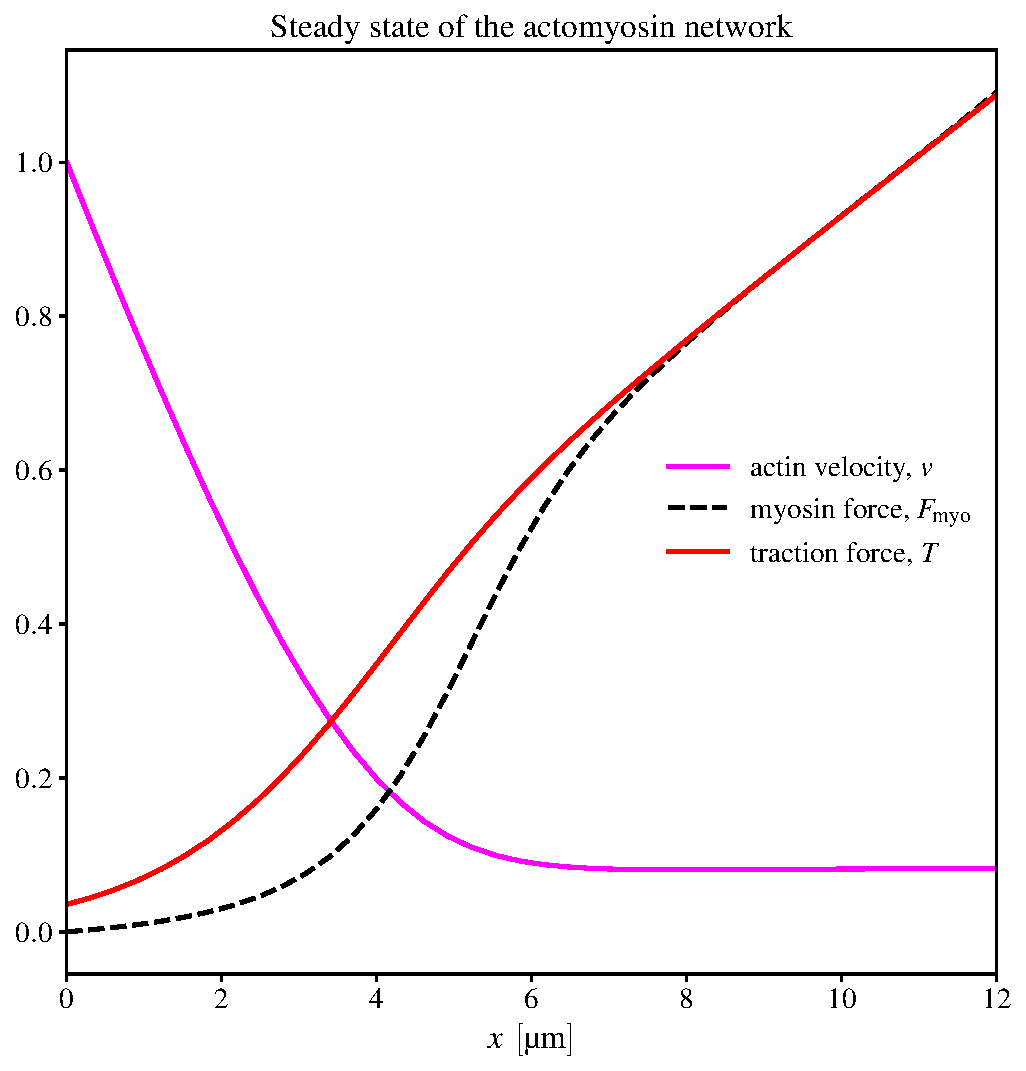
\includegraphics[width=\linewidth]{../.figures/steady_state_og_highF.pdf}
    \caption{\label{fig:steady_highF}}
    \end{subfigure}%
    \hfill
    \begin{subfigure}{0.3\textwidth}
    \centering
    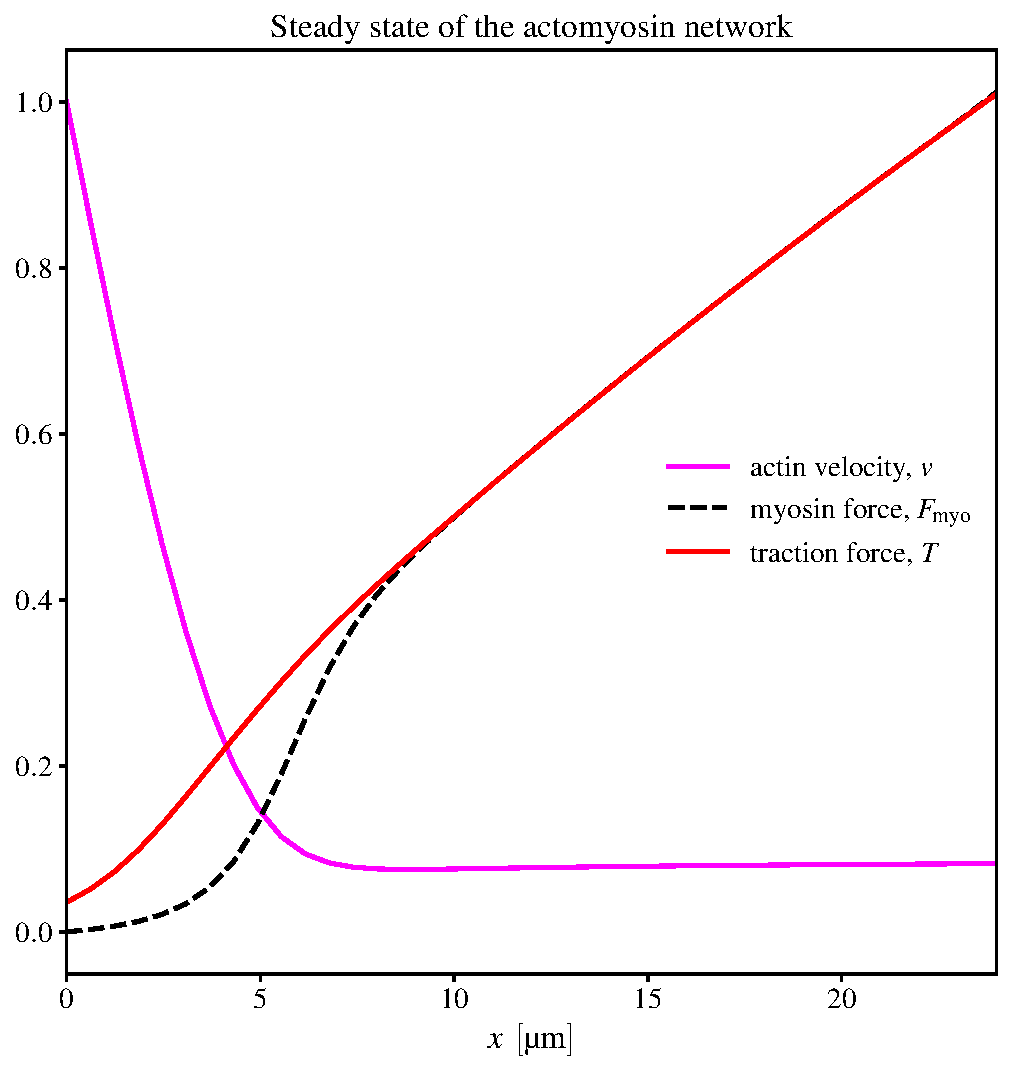
\includegraphics[width=\linewidth]{../.figures/steady_state_og_longL.pdf}
    \caption{\label{fig:steady_longL}}
    \end{subfigure}
    \caption{\label{fig:sim_steady}
    Representative output of the steady state of the actomyosin network from Ref.~\cite{craig_membrane_2012}. The pink line represents the retrograde actin flow speed from the leading edge, \(x=\qty{0}{\micro\meter}\), to the trailing edge, \(x=\qty{12}{\micro\meter}\). The black dashed line represents the contractile forces from myosin. The red line represents the traction forces arising from actin adhesion to the substrate. Under these conditions the GC is moving in the \(-x\) direction. Figure~\ref{fig:steady_og} represents the conditions used throughout the investigation. Figure~\ref{fig:steady_highF} represents a steady state for Myosin with twice the strength and Figure~\ref{fig:steady_longL} represents a steady state for a actomyosin network of \(\qty{24}{\micro\meter}\).
    }
\end{figure}

In addition to the features of this model we introduce MTs protruding from the axon via Dynein sliding forces. After the network has reached a steady state, we permit MTs to enter the GC through Dynein sliding forces and MT polymerization. Here we introduce two distinct behaviors for testing:
\begin{enumerate}
\item crosslinker proteins bind primarily to the plus-end of the MT effectively resulting in a single point of contact with the actomyosin network;
\item crosslinker proteins bind uniformly to the MT resulting in multiple contact points across the actomyosin network.
\end{enumerate}

% model figure
\begin{figure}
    \centering
    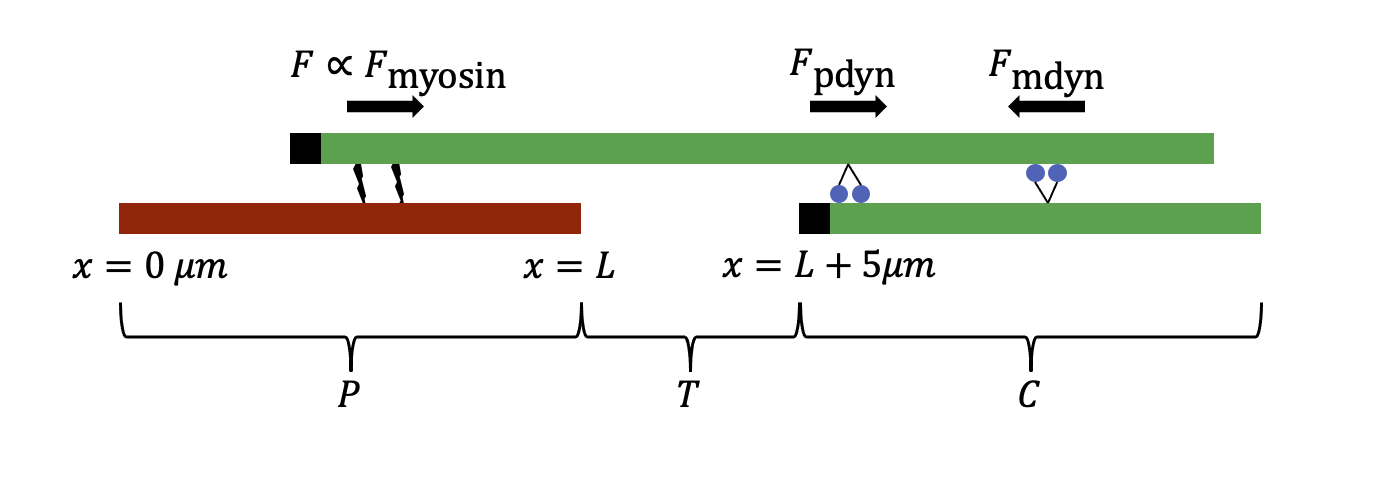
\includegraphics[width=0.9\textwidth]{figures/model/model.png}
    \caption{\label{fig:main_model}
        The one-dimensional model of the GC under study. Labelled below are the P, T, and C regions of the GC. In the P region we model an actomyosin network as in Ref.~\cite{craig_membrane_2012}. Here, crosslinker proteins bind to the protruding MT and exert a force proportional to the velocity of myosin at the binding location. The length of this region can be tuned but it set to \(L=\qty{12}{\micro\meter}\). In the \(\qty{5}{\micro\meter}\) T region no protein binding occurs. In the C region Dynein motors bind between the single MT protruding into the GC and an array of axonal MTs assumed to be stabilized against motion by a network of crosslinkers.
    }
\end{figure}

The simulation begins with the actomyosin network reaching a steady state as described by Ref.~\cite{craig_membrane_2012}. Once in a steady state we move to an agent based model simulating the action of a single MT protruding into the GC. We simulate the interactions of this MT and motor proteins described in Figure~\ref{fig:main_model} over a characteristic time of \(t=\qty{100}{\second}\). This time is obtained by calculating the time it takes for an actin filament to traverse the actomyosin network. On time-scales below this we assume the actomyosin network will remain in its steady state.

\end{block}

%------------------------------------------------
% content block
\begin{block}{Results}

% comparison between model 1 and 2 for MT trajectories and total compressive load
% three side-by-side figures
\begin{figure}
    \begin{subfigure}{0.45\textwidth}
    \centering
    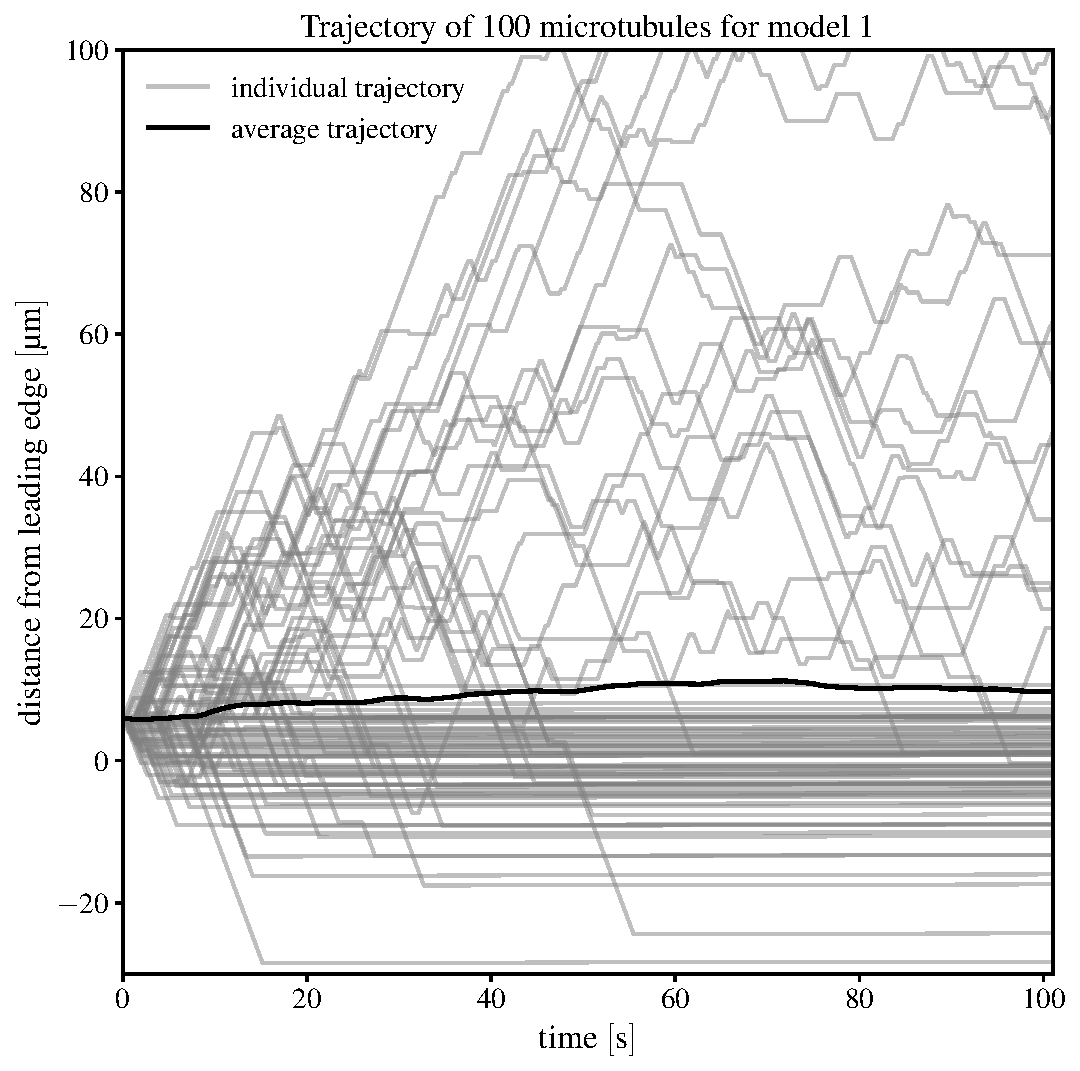
\includegraphics[width=\linewidth]{../.figures/mt_trajectory_m1.pdf}
    \caption{\label{fig:traj_m1}}
    \end{subfigure}%
    \hfill
    \begin{subfigure}{0.45\textwidth}
    \centering
    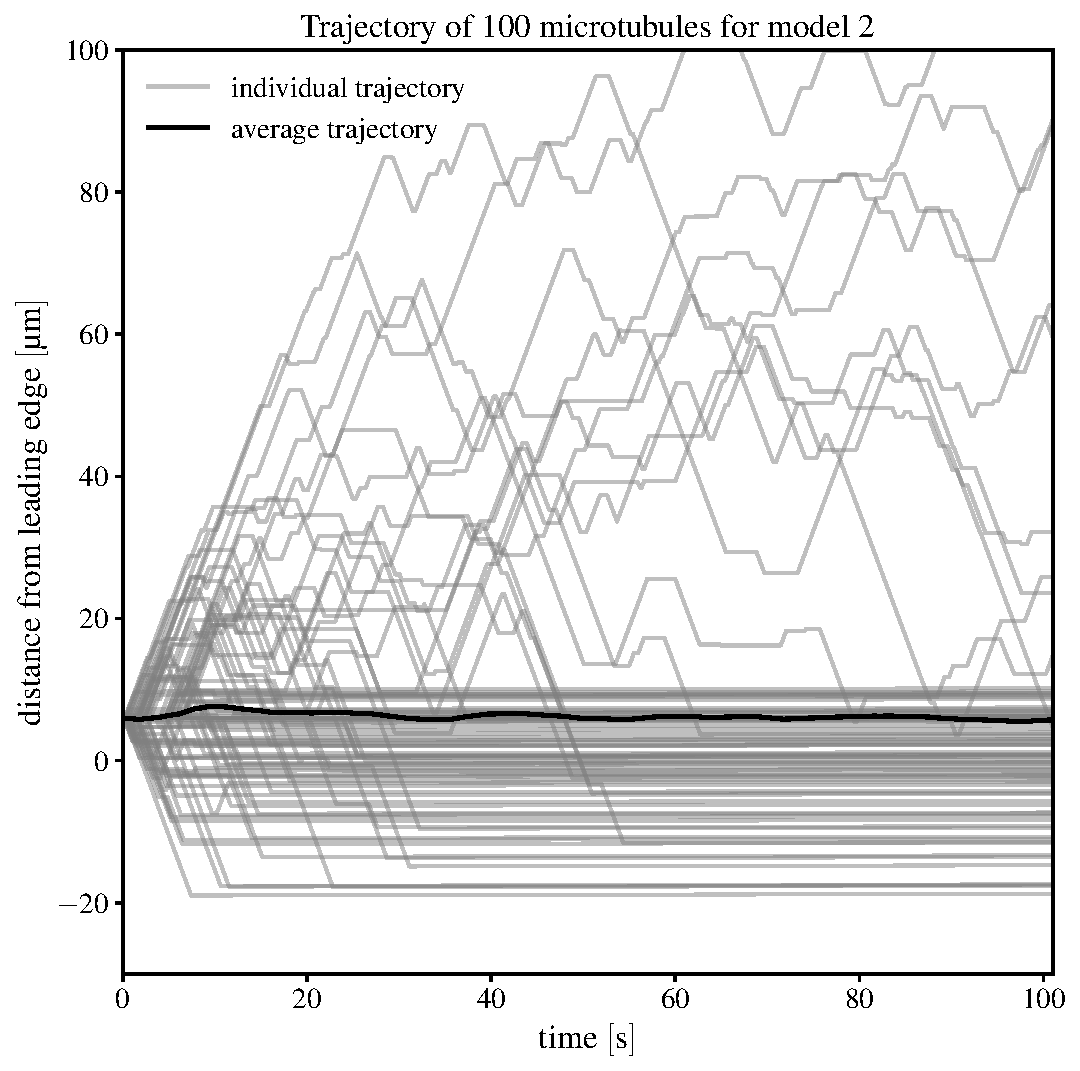
\includegraphics[width=\linewidth]{../.figures/mt_trajectory_m2.pdf}
    \caption{\label{fig:traj_m2}}
    \end{subfigure}%
    \hfill
    \caption{\label{fig:three_comp}
        Comparisons between model 1 and model 2 in trajectories and compressive forces. Figure~\ref{fig:traj_m1} and~\ref{fig:traj_m2} indicate the trajectories of individual MTs as well as the average trajectory for each model.
    }
\end{figure}

\end{block}

\end{column}
\separatorcolumn%


%-----------------------------------------------------------------------------%
% third column of content
\begin{column}{\colwidth}

%------------------------------------------------
% content block
\begin{block}{Results}

% show close up comparison figure
\begin{figure}
    \centering
    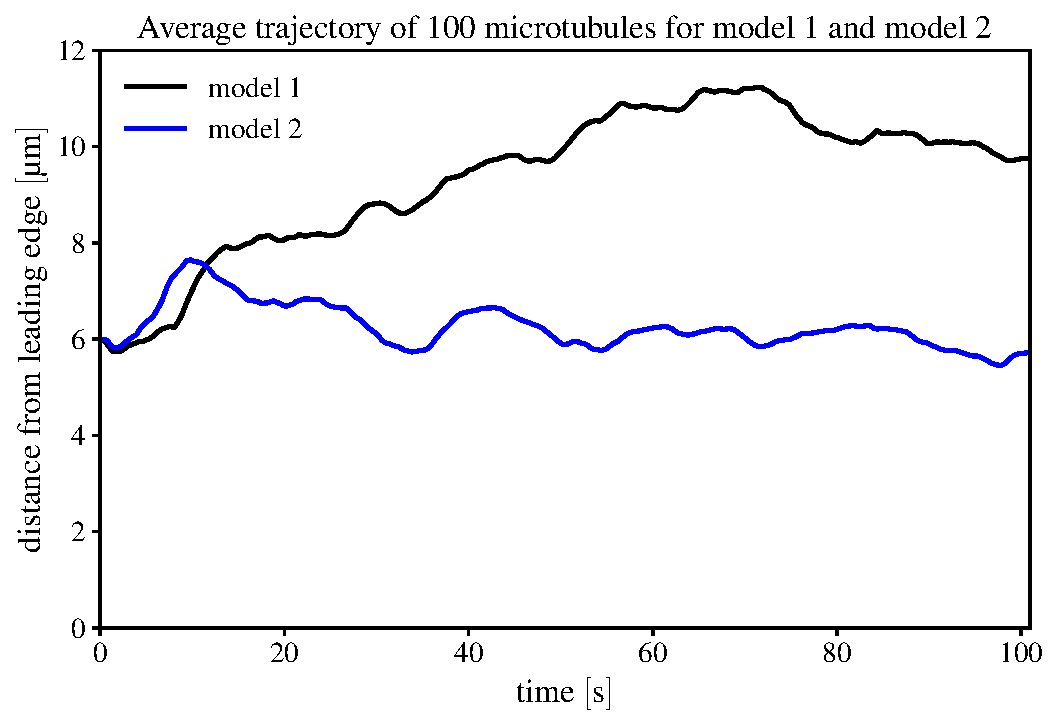
\includegraphics[width=0.4\textwidth]{../.figures/mt_trajectory_average_closeup.pdf}
    \caption{\label{fig:traj_comp}
        In black, the average trajectory of model 1 MTs from Figure~\ref{fig:traj_m1}. In blue, the average trajectory of model 2 MTs from Figure~\ref{fig:traj_m2}. The vertical axis has been limited to the spacial extent of the actomyosin network.
    }
\end{figure}

A qualitative inspection of Figure~\ref{fig:traj_m1} and~\ref{fig:traj_m2} might indicate a difference in the average trajectory of model 1 and model 2 type binding. Figure~\ref{fig:traj_comp} further illustrates this difference. The position indicated is the position of the plus-end of the MT on a coordinate system illustrated in Figure~\ref{fig:main_model}. Of particular note in Figure~\ref{fig:traj_comp} is that model 1 MTs tend to drift out of the network while model 2 MTs remain roughly in place and may even be drifting inward.

\begin{figure}
    \centering
    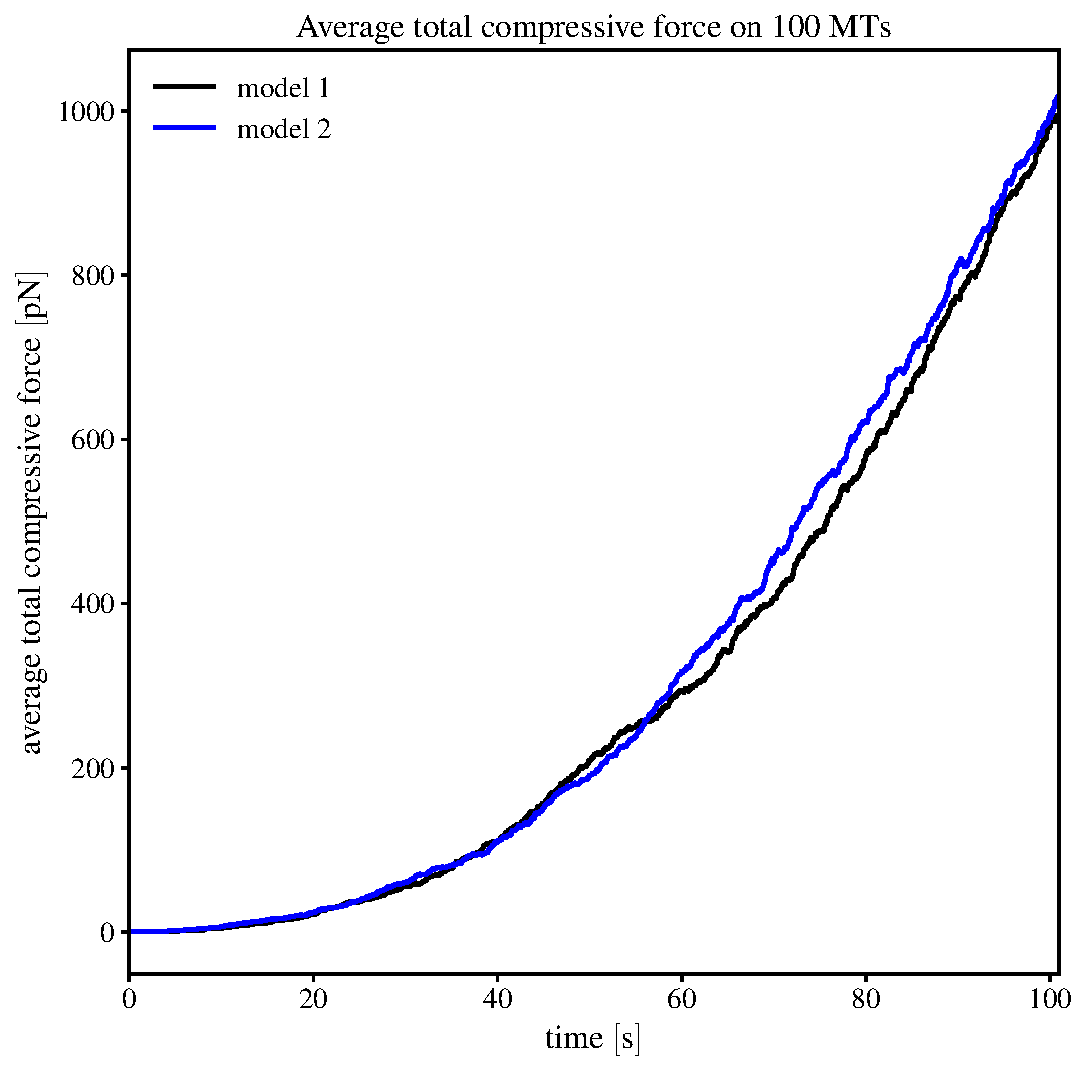
\includegraphics[width=0.4\textwidth]{../.figures/average_compressive_force.pdf}
    \caption{\label{fig:comp_force}
        The average axially directed force on the MT as a consequence of myosin contractile forces pushing in the \(+x\) direction and Dynein motors pushing in the \(-x\) direction.
    }
\end{figure}

Figure~\ref{fig:comp_force} illustrates how the stress placed on the MTs might develop with time in the actomyosin network. Model 1 and model 2 MTs do not exhibit significant difference in how their compressive forces develop. It should be noted that this model does not currently allow MTs to break. Should breaking under load be implemented it is very likely that the MTs would have bent and broken before reaching the peak force of \(\approx \qty{1}{\nano\newton}\)~\cite{takasone_flexural_2002}.

\end{block}

%------------------------------------------------
% conclusion block
\begin{block}{Conclusion}

We began with an existing model studying the treadmilling effect of the actomyosin network in the GC of axons~\cite{craig_membrane_2012}. By incorporating a simple agent-based interaction of a single MT protruding into the growth cone and interacting with the actomyosin network we were able to test two different models of crosslinker binding. Our results indicate that there may exist observable differences in the spatial distribution of the MTs which may be useful in experimentally testing these models.

\end{block}

%------------------------------------------------
% future work block
\begin{block}{Future Work}

This model currently only considers a single interaction time-scale between the actomyosin network and the protruding MTs. There are unexplored behaviors not observed due to the lack of feedback from the effect of an MT dragging against the actomyosin treadmill. An agent based model that updates both the MTs and the actomyosin network at the same time steps would be able to capture this behavior in a way that the current model does not. Furthermore, this current model does not consider bending and snapping of MTs which is known to contribute both to GC forces and to the production of distally located short MTs. Implementing breaking of MTs as a consequence of compressive forces is essential in reaching grater understanding. Already this model predicts compressive forces beyond what MTs are likely able to handle~\cite{takasone_flexural_2002}.

\end{block}

%------------------------------------------------
% reference block
\begin{block}{References}
\begin{multicols}{2}
\fontsize{16pt}{12pt}\selectfont
% \nocite{craig2015pb, craig2012bj, devincentiis2020jn, kalil2005con, nedelec1997n13, raffa2023scdb, sanchez-huertas2021fmn}
\bibliographystyle{plain}
% \bibliography{../proposal/axon_growth2.bib}
\bibliography{poster_refs.bib}
\end{multicols}
\end{block}

\end{column}
\separatorcolumn%

\end{columns}
\end{frame}
\end{document}
